\documentclass[binding=0.6cm,Lau,noexaminfo]{sapthesis}
\usepackage[italian]{babel}
\usepackage[utf8]{inputenc}
\usepackage[autostyle,italian=guillemets]{csquotes}
\usepackage[style=numeric,backend=biber]{biblatex}
\addbibresource{sample.bib}

\usepackage{listings}
\lstdefinelanguage{Gherkin}{
	morekeywords = {
		Given,
		When,
		Then,
		And,
		Scenario,
		Feature,
		But,
		Background,
		Scenario Outline,
		Examples
	},
	sensitive=true,
	morecomment=[l]{\#},
	morestring=[b]",
	morestring=[b]'
}
\usepackage{graphicx}
\usepackage{array}
\usepackage{float}
\usepackage{microtype}
\usepackage{parskip}
\usepackage[section]{placeins}
\usepackage{hyperref}
\hypersetup{pdftitle={La mia tesi},pdfauthor={Giacomo Colizzi Coin}}
\makeatletter
\newcommand\urlfootnote@[1]{\footnote{\url@{#1}}}
\DeclareRobustCommand{\urlfootnote}{\hyper@normalise\urlfootnote@}
\makeatother

% \title{Game\_on: progetto ed implementazione di una piattaforma di condivisione di videogiochi e di gioco online}
\title{Game on: piattaforma per condividere videogiochi}
\author{Giacomo Colizzi Coin}
\IDnumber{1794538}
\course{Ingegneria informatica}
\courseorganizer{Facoltà di ingegneria dell'informazione, informatica e statistica}
\AcademicYear{2019/2020}
\copyyear{2020}
\advisor{Prof. Leonardo Querzoni}
\authoremail{colizzicoin.1794538@studenti.uniroma1.it}

\begin{document}
\frontmatter
\maketitle

\tableofcontents

\mainmatter

\chapter{Introduzione}

Nella società attuale, programmare sta diventando sempre più comune e
alla portata di tutti.
% Inserire statistiche qui
Uno degli ambiti di interesse più comuni nella fascia di età citata è
quello dei videogiochi. Esistono molte piattaforme in cui un utente
può scegliere un gioco e giocarci liberamente, ed esistono anche
piattaforme che permettono di caricare i propri giochi. Queste
piattaforme richiedono però di avere dei requisiti particolari.
Inoltre, la velocità sempre crescente delle connessioni internet ha
permesso ai servizi di streaming di avere sempre più successo.

In questo contesto nasce l'idea di questa tesi.
Il progetto ha come obiettivo la creazione di una piattaforma per la
condivisione di videogiochi. Gli utenti di questa piattaforma possono
condividere con gli altri utenti i giochi da loro sviluppati. Tutti i
giochi caricati sulla piattaforma sono giocabili da ogni utente.
Infine, come utente, è possibile condividere le proprie esperienze di
gioco votando, commentando, invitando amici e altro.


\chapter{Requisiti, tecnologie e metodologie}

\section{Funzionalità offerte}

Come detto in precedenza, il sistema informativo progettato intende offrire agli utenti la possibilità di codividere, modificare e giocare ai videogiochi da loro sviluppati.
\newline
Chiunque voglia usufruire di questo servizio può creare un proprio account all'interno del sistema. I giochi caricati saranno visibili e giocabili da tutti gli altri utenti.
\newline
Per entrare nello scpecifico, passiamo ora alla descrizione delle funzionalità principali. Per comodità di esposizione, nella descrizione di queste divideremo l'analisi in sezioni e faremo riferimento diretto alle \textit{user stories}

\subsection{Sezione utenti}

Un visitatore del sito web che intende accedere al servizio deve ottenere le autorizzazione del sistema creando un account personale. Alla registrazione vengono richiesti un \textit{username}, un'\textit{email} valida e una \textit{password} per gli accessi futuri. In alternativa può registrarsi attraverso l'utilizzo della tecnologia \textit{OAuth}. Da questo momento in poi sarà definito \textit{giocatore}. Dopo aver confermato la sua registrazione, potrà accedere nuovamente al servizio fornendo le proprie credenziali. Avrà anche la possibilità di modificare le informazioni relative al proprio account.
\newline
Le user stories relative agli utenti sono le seguenti:
\textit{
\begin{enumerate}
\item Come visitatore, voglio creare un nuovo account, in modo che il sistema possa ricordarsi di me.
\item Come giocatore, voglio effettuare il login, in modo che possa interagire col sistema.
\item Come giocatore, voglio poter effettuare l'accesso con un account Google o Github.
\item Come giocatore, voglio poter terminare la sessione, così che il mio account sia protetto da usi non autorizzati.
\item Come giocatore, voglio poter modificare i dati del mio account, così che lo possa mantenere aggiornato.
\end{enumerate}
}

\begin{figure}[h!]
\centering
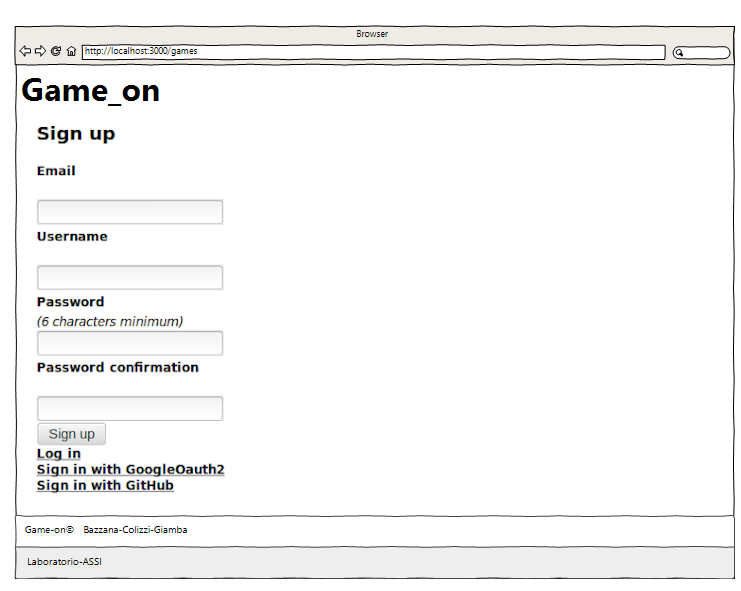
\includegraphics[width=0.45\textwidth]{mockup_registration}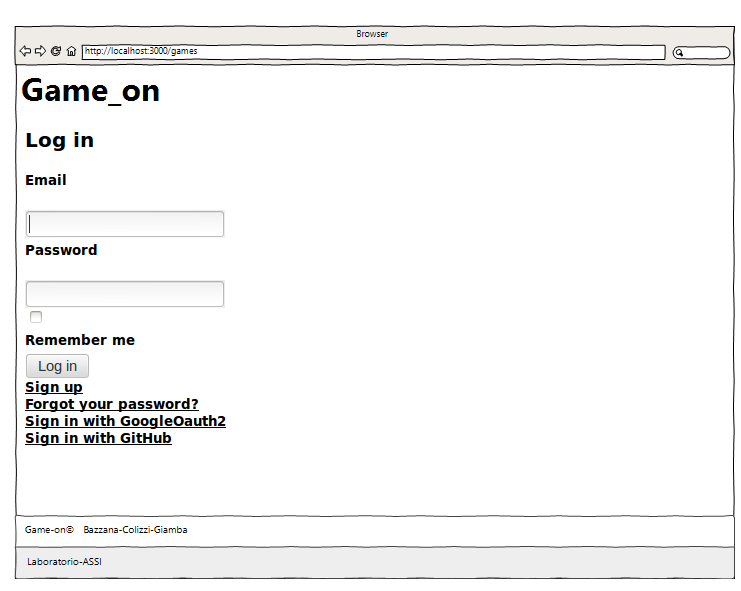
\includegraphics[width=0.45\textwidth]{mockup_login}
\caption{Mockup relativi alle user stories 1, 2 e 3}
\end{figure}

\subsection{Sezione giochi}

Ogni utente (anche un visitatore) può vedere l'elenco dei giochi presenti sulla piattaforma e effettuare ricerche all'interno di esso, mentre solo i giocatori possono giocare, caricare giochi e modificare o eliminare i propri. Per caricare un suo gioco sviluppato con \textit{Unity} un giocatore deve compilare il form presente in una pagina dedicata. Ogni giocatore può esprimere una preferenza su un gioco o fornire un voto positivo o negativo. Può inoltre vedere la lista dei suoi giochi preferiti.
\newline
Le user stories relative a queste funzionalità sono le seguenti:

\textit{
\begin{enumerate}
\item Come utente generico, voglio visualizzare l'elenco di tutti i giochi aggiunti nella piattaforma dagli altri giocatori.
\item Come utente generico,
voglio cercare un gioco specifico cercandolo per nome o per categoria, in modo che possa cercare solo ciò che mi interessa.
\item Come utente generico,
voglio ordinare i risultati di una ricerca, in modo che possa avere i risultati disposti secondo vari criteri.
\item Come giocatore, voglio inserire un gioco nella piattaforma, in modo che sia visibile agli altri utenti.
\item Come giocatore, voglio rimuovere un mio gioco dalla piattaforma, in modo che non sia più disponibile su di essa.
\item Come utente generico, voglio vedere le informazioni di un gioco.
\item Come giocatore, voglio giocare a un gioco.
\item Come giocatore proprietario di un gioco, voglio modificare la descrizione del gioco, così che lo possa mantenere aggiornato.
\item Come giocatore proprietario di un gioco, voglio rilasciare una patch del gioco, così da mostrare solo la versione più aggiornata.
\item Come giocatore, voglio assegnare o rimuovere un like o un dislike ad un gioco, in modo da fornire un feedback pubblico allo sviluppatore.
\item Come giocatore, voglio aggiungere/rimuovere un gioco ai miei preferiti, in modo che lo possa trovare nella mia lista preferiti.
\item Come giocatore, voglio visualizzare una pagina con tutti i miei giochi preferiti, in modo che siano tutti raggruppati in un unico posto.
\end{enumerate}
}

\begin{figure}[h!]
\centering
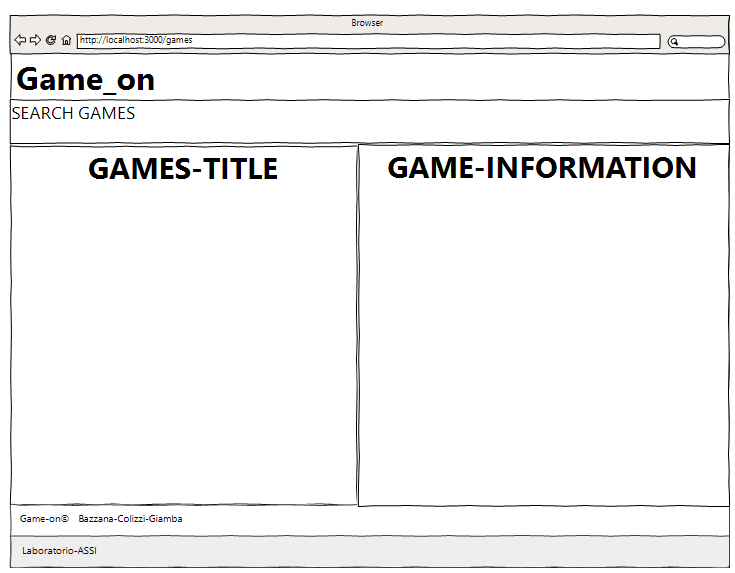
\includegraphics[width=0.45\textwidth]{mockup_games}
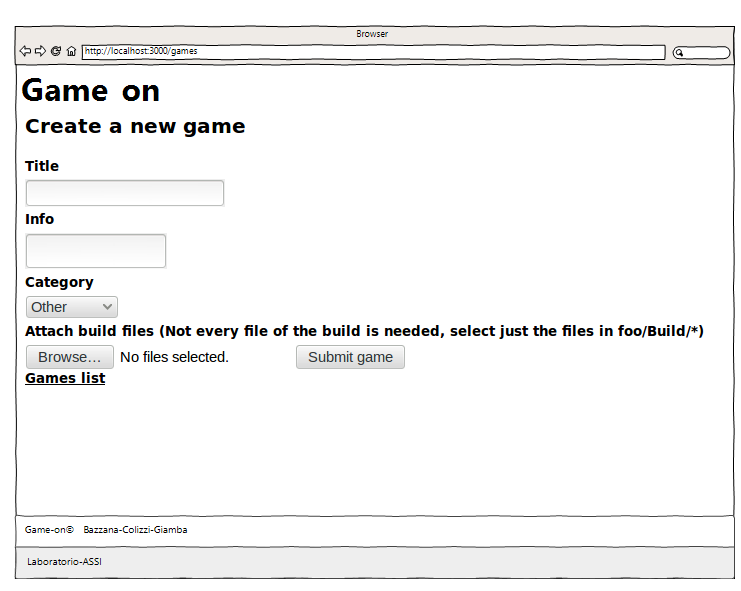
\includegraphics[width=0.45\textwidth]{mockup_add_game}
\caption{Mockup relativi alle user stories 1 e 4}
\end{figure}


\section{Metodologia utilizzata di conduzione del progetto ed organizzazione del lavoro}

Il gruppo di lavoro è formato da tre componenti: Davide Bazzana,
Giacomo Colizzi Coin e Renato Giamba.
\newline
\newline
Lo sviluppo del progetto è stato organizzato seguendo la metodologia
ASD (\textit{agile software development}).

Il calendario è stato suddiviso in iterazioni, in modo da definire
quante e quali user stories dovevano essere sviluppate in un certo
periodo di tempo. Subito dopo aver definito le user stories da
svluppare, esse sono state suddivise in gruppi, ciascuno affidato ad
una iterazione. Nella prima parte dello sviluppo, la durata di
ciascuna iterazione è stata di 3 settimane, successivamente però tale
durata è stata ridotta a 2 settimane, per accelerare lo sviluppo e
concludere il progetto rispettando la data di consegna che il gruppo
si era inizialmente proposto.  Ad ogni scadenza di una iterazione, ed
inizio di quella successiva, il gruppo si riuniva per discutere dei
traguardi raggiunti e di quelli da raggiungere in futuro. Lo scopo
principale di queste riunioni era infatti quello di assegnare a
ciascun componente del gruppo un insieme di user stories appartenti
alla successiva iterazione.  Questa scelta veniva fatta in base alla
propensione dei singoli componenti e alle competenze di ciascuno di
essi, sia acquisite in altre occasioni, sia acquisite durante lo
sviluppo del progetto stesso. Questo modus operandi ha fatto sì che i
vari componenti del gruppo, pur continuando a mantenere una visione
chiara del funzionamento complessivo dell'applicazione, si siano
specializzati in un suo ambito specifico.

\subsection{Servizi di terze parti utilizzati}

Per gestire ed analizzare l'andamento dello sviluppo del progetto è
stato utilizzato il tool \textit{PivotalTracker}.

Questo tool ha permesso al gruppo di tenere traccia di tutte le user
stories e delle loro relative informazioni: il contenuto della user
story, il suo stato di sviluppo (unstarted, started, finished, delivered,
rejected, accepted), l'iterazione alla quale faceva riferimento, il
componente responsabile del suo sviluppo, il livello di difficoltà, ed
altro. Per tutta la durata del progetto, ciascun componente aveva la
possibilità di consultare e modificare tali informazioni.

Infine, \textit{PivotalTracker}, ha reso possibile valutare in tempo
reale le informazioni relative all'andamento dello sviluppo, come la
sua velocità e volatilità.
\newline
\newline
Per il controllo di versione è stato scelto il software \textit{Git},
mentre, come servizio di hosting per la repository del progetto, è
stato scelto \textit{GitHub}.

La metodologia impiegata dal gruppo per l'utilizzo dei branch della
repository è stata quella di creare un branch per ciascuna user story
in sviluppo e di mantenere un branch chiamato ``\textit{master}'' come
branch di mantenimento di una versione stabile.

La procedura di controllo del nuovo software prodotto invece, è stata
quella di \textit{peer review}. Infatti, ogni volta che un componente
del gruppo completava l'implementazione di una user story, sottoponeva
il suo lavoro al giudizio degli altri. Questa procedura veniva svolta
facendo uso del meccanismo di pull request offerto da
\textit{GitHub}. Se il resto dei componenti del gruppo riteneva il
lavoro svolto adeguato, la \textit{pull request} veniva accettata e si
procedeva col \textit{merging} del branch in questione con il branch
``\textit{master}'', altrimenti, il componente, o i componenti, che
non ritenevano il lavoro svolto sufficiente, commentavano la
\textit{pull request} evidenziando eventuali errori da correggere o
miglioramenti da apportare.
\newline
\newline
Infine è stata sfruttata la possibilità di integrare un progetto su
\textit{PivotalTracker} con una repository su \textit{GitHub}.

Con questa funzionalità abilitata, tutti gli avanzamenti di un branch
relativo ad una user story venivano comunicati da \textit{GitHub} a
\textit{PivotalTracker}, provocando così l'aggiornamento automatico
dello stato della user story su \textit{PivotalTracker}.

\subsection{Statistiche di sviluppo}

Il progetto è iniziato il 21 marzo 2020 e finito il 16 settembre
2020, con una durata totale di 25 settimane e 5 giorni.
\newline
\newline
La tabella seguente mostra alcune statistiche sul contributo di
ciascun componente del gruppo. Pur riportando il numero esatto di
commit, file e righe prodotte da ciascuno, i seguenti dati sono
indicativi. Infatti, ad esempio, una percentuale non indifferente del
numero di file e linee indicate, non costituisce un contributo diretto
del componente, bensì deriva dalle gemme e dai file di terze parti
utilizzati, come quelli prodotti da \textit{Unity 3D} per il
gioco di test ``\textit{Kloby}''.

\vspace{1cm}
\begin{tabular}{l|r|r|r}
  \textbf{Developer} & \textbf{Commits} & \textbf{Files changed} & \textbf{Total lines} \\
  \hline
  Davide Bazzana & 111 & 366 & 7428 \\
  \hline
  Giacomo Colizzi Coin & 88 & 506 & 2680 \\
  \hline
  Renato Giamba & 42 & 183 & 1110 \\
  \hline
\end{tabular}


\chapter{Analisi concettuale del sistema}

In questo capitolo verrano mostrati gli aspetti delo sviluppo della piattaforma per quanto riguarda il progetto della base di dati.\cite{DB}

\section{Analisi dei requisiti}

Per progettare una base di dati è necessario comprendere la realtà da rappresentare effettuando la cosiddetta raccolta dei requisiti, cioè l'individuazione dei problemi che l'applicazione deve risolvere tenendo presenti sia gli aspetti statici (i dati) che quelli dinamici (le operazioni sui dati).\\

Segue un elenco dei requisiti della base di dati per lo specifico sistema informatico. 

\hangindent=1cm
\hangafter=1
{\scshape I giocatori.} Di ogni giocatore interessa l'email (che deve essere unica), l'username, la password se effettua il login standard, il provider se effettua il login con OAuth e il ruolo che gli è stato assegnato. Ogni giocatore può seguire o essere seguito da altri giocatori. Ogni giocatore può pubblicare dei giochi, può pubblicare recensioni, votare positivamente o negativamente e aggiungere ad una lista preferiti dei giochi. Per il servizio typingDNA è necessario inoltre conoscere il numero di login effettuati, se il giocatore è stato registrato nel sistema di typingDNA e quanti tentativi ha a disposizione prima che gli venga bloccato l'account.

\hangindent=1cm
\hangafter=1
{\scshape I giochi.} Di ogni gioco interessa il titolo, la descrizione, la categoria, l'utente che l'ha pubblicato e opzionalmente la versione. Ogni gioco è composto da un solo blocco di file di build. I giochi possono essere recensiti, votati e resi preferiti da più giocatori contemporaneamente.

\hangindent=1cm
\hangafter=1
{\scshape I file di build} sono un blocco composto da 5 file specifici del framework Unity con il quale i giochi devono essere programmati per poter funzionare sulla piattaforma.

\hangindent=1cm
\hangafter=1
{\scshape Le recensioni.} Di ogni recensione interessa la data di pubblicazione, il testo, l'utente che l'ha pubblicata e il gioco a cui si riferisce.

\section{La progettazione concettuale}
Lo scopo della progettazione concettuale è quello di rappresentare le specifiche informali ricavabili dai requisiti in modo schematico. Questo schema prende il nome di schema ER (Entità-Relazione). Si tratta di un modello concettuale ad alto livello di astrazione che, quindi, non tiene conto degli aspetti implementativi.

\subsection{Lo schema Entità-Relazione}
Oltre allo schema ER è necessario riportare delle tabelle descrittive per le entità, relazioni e attributi.


\begin{table}[hbt!]
    \centering
    \begin{tabular}{ m{0.15\textwidth} m{0.24\textwidth} m{0.24\textwidth} m{0.24\textwidth} }
        \hline
        \textbf{Entità} & \textbf{Descrizione} & \textbf{Attributi} & \textbf{Identificatori} \\
        \hline
        \textbf{Giocatore} & Utente registrato nell'applicazione & email, password, provider, ruolo, numero di login, registrato su typingDNA, tentativi typingDNA & \{email\} \\
        \hline
        \textbf{Gioco} & Gioco caricato sulla piattaforma & game id, titolo, descrizione, categoria, versione & \{game id\} \\
        \hline
        \textbf{Recensione} & Recensione pubblicata da un giocatore per un gioco & data, testo & \{giocatore, gioco\} \\
        \hline
        \textbf{File di build} & Blocco di file di build di un gioco &  & \{gioco\} \\
        \hline
        \textbf{File} & Il singolo file di build & file id, nome, contenuto & \{file id\} \\
    \end{tabular}
    \caption{Entità}
\end{table}

\begin{table}[hbt!]
    \centering
    \begin{tabular}{ m{0.17\textwidth} m{0.18\textwidth} m{0.18\textwidth} m{0.18\textwidth} m{0.18\textwidth} }
        \hline
        \textbf{Relazione} & \textbf{Descrizione} & \textbf{Componenti} & \textbf{Attributi} & \textbf{Identificatori} \\
        \hline
        \textbf{Pubblicazione} & Ogni gioco è pubblicato da un utente & Giocatore\newline Gioco & data & \{gioco\} \\
        \hline
        \textbf{Pubblica} & Un giocatore può pubblicare una recensione & Giocatore\newline Recensione &  & \{recensione\} \\
        \hline
        \textbf{RG} & Ogni recensione è legata ad un gioco & Recensione\newline Gioco & & \{recensione\} \\
        \hline
        \textbf{Preferito} & Un giocatore può aggiungere un gioco ai suoi preferiti & Giocatore\newline Gioco & & \{giocatore, gioco\} \\
        \hline
        \textbf{Relazione} & Un giocatore può seguirne un altro & Giocatore\newline Giocatore & & \{seguace, seguito\} \\
        \hline
        \textbf{Voto} & Voto espresso da un giocatore per un gioco & Giocatore\newline Gioco & valore & \{giocatore, gioco\} \\
        \hline
        \textbf{Composto da} & Un gioco può avere allegato un blocco di file & Gioco\newline File di build & & \{file di build\} \\
        \hline
        \textbf{Comprende} & Ogni blocco di file di build è composto da 5 file & File di build\newline File &  & \{file\} \\
    \end{tabular}
    \caption{Relazioni}
\end{table}

\begin{table}[hbt!]
    \centering
    \begin{tabular}{m{0.18\textwidth} m{0.24\textwidth} m{0.19\textwidth} m{0.32\textwidth}}
        \hline
        \textbf{Attributo} & \textbf{Entità/Relazione} & \textbf{Dominio} & \textbf{Descrizione} \\
        \hline
        \textbf{Email} & Giocatore & String & L'email del giocatore \\
        \hline
        \textbf{Ruolo} & Giocatore & String & Il ruolo del giocatore nell'applicazione \\
        \hline
        \textbf{Numero di login} & Giocatore & Integer & Numero di accessi al sito per il giocatore \\
        \hline
        \textbf{Registrato su typingDNA} & Giocatore & Boolean & Un giocatore è registrato su typingDNA quando ha fatto vari login sulla piattaforma \\
        \hline
        \textbf{Tentativi typingDNA} & Giocatore & Integer & Numero di tentativi di autenticazione con typingDNA \\
        \hline
        \textbf{Password} & Giocatore & String & La password per accedere con il proprio account \\
        \hline
        \textbf{Provider} & Giocatore & String & Il provider del servizio OAuth per il giocatore \\
        \hline
        \textbf{Data} & Pubblicazione & Date & La data di pubblicazione di un gioco \\
        \hline
        \textbf{Data} & Recensione & Date & La data di pubblicazione di una recensione  \\
        \hline
        \textbf{Testo} & Recensione & Text & Testo di una recensione \\
        \hline
        \textbf{Valore} & Voto & Integer & Voto dato ad un gioco. Può essere +1 o -1 \\
        \hline
        \textbf{Game ID} & Gioco & Integer & Numero identificativo di un gioco \\
        \hline
        \textbf{Titolo} & Gioco & String & Titolo di un gioco \\
        \hline
        \textbf{Descrizione} & Gioco & Text & Descrizione di un gioco \\
        \hline
        \textbf{Categoria} & Gioco & String & La categoria di cui fa parte un gioco \\
        \hline
        \textbf{Versione} & Gioco & String & La versione di patch di un gioco \\
        \hline
        \textbf{File ID} & File & Integer & Numero che identifica un file \\
        \hline
        \textbf{Nome} & File & String & Nome del file \\
        \hline
        \textbf{Contenuto} & File & BLOB & Contenuto effettivo del file che permette l'esecuzione del gioco \\
    \end{tabular}
    \caption{Attributi}
\end{table}

\begin{figure}[hbt!]
    \centering
    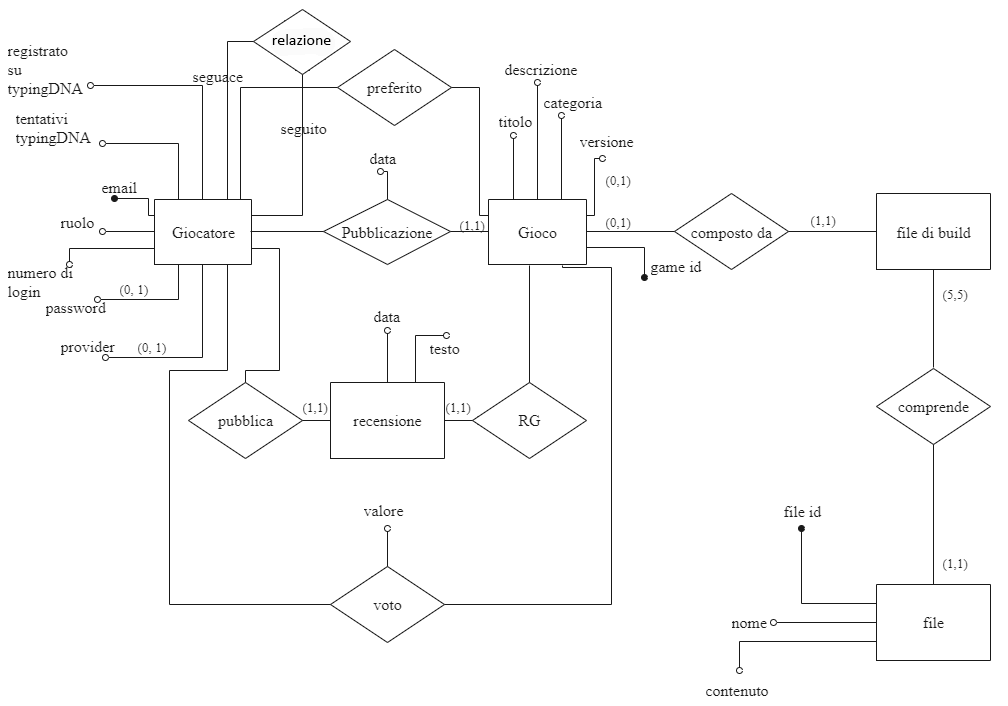
\includegraphics[angle=-90, width=\textwidth]{schemaER}
    \caption{Schema ER}
\end{figure}

\begin{table}[hbt!]
    \centering
    \begin{tabular}{m{0.18\textwidth} m{0.24\textwidth} m{0.55\textwidth}}
        \hline
        \textbf{Relazione} & \textbf{Componenti} & \textbf{Vincoli di cardinalità}\\ \hline
        \textbf{Relazione} & Seguace & Ogni giocatore può essere seguace di 0 o più giocatori \\ \cline{2-3}
        & Seguito & Ogni giocatore può essere seguito da 0 o più giocatori \\ \hline
        \textbf{Pubblicazione} & Giocatore & Ogni giocatore può pubblicare 0 o più giochi \\ \cline{2-3}
        & Gioco & Ogni gioco è pubblicato da uno e un solo giocatore \\ \hline
        \textbf{Pubblica} & Giocatore & Ogni giocatore può pubblicare 0 o più recensioni \\ \cline{2-3}
        & Recensione & Ogni recensione è pubblicata da uno e un solo giocatore \\ \hline
        \textbf{RG} & Recensione & Ogni recensione appartiene ad uno e un solo gioco \\ \cline{2-3}
        & Gioco & Ogni gioco può avere 0 o più recensioni \\ \hline
        \textbf{Voto} & Giocatore & Ogni giocatore può esprimere 0 o più voti \\ \cline{2-3}
        & Gioco & Ogni gioco può ricevere 0 o più voti \\ \hline
        \textbf{Preferito} & Giocatore & Ogni giocatore può aggiungere ai preferiti 0 o più giochi \\ \cline{2-3}
        & Gioco & Ogni gioco può essere preferito da 0 o più giocatori \\ \hline
        \textbf{Composto da} & Gioco & Ogni gioco ha allegato 0 o un blocco di file \\ \cline{2-3}
        & File di build & Ogni blocco di file di build è legato ad uno e un solo gioco \\ \hline
        \textbf{Comprende} & File di build & Ogni blocco di file di build è costituito da 5 file \\ \cline{2-3}
        & File & Ogni file appartiene ad un solo blocco di file di build \\
    \end{tabular}
    \caption{Vincoli di cardinalità}
\end{table}

\FloatBarrier
\subsection{Le \emph{business rules}}
Lo schema ER è fondamentale per comprendere la struttura astratta dell'applicazione, ma ha dei limiti. Non tutte le problematiche sono codificabili con questo schema e perciò è necessario aggiungere dei vincoli esterni (spesso chiamati \emph{business rules}) che lo completano.

\begin{table}[hbt!]
    \begin{tabular}{p{1cm} m{0.88\textwidth}}
        \hline
        & \textbf{Vincoli d'integrità non esprimibili nel diagramma ER} \\
        \hline 
        \textbf{1} & Ogni istanza di Giocatore non può partecipare contemporaneamente alla stessa istanza di following con il ruolo di Seguito e Seguace. \\ \hline
        \textbf{2} & Per ogni istanza di Giocatore, almeno uno tra i campi \emph{password} e \emph{provider} deve essere presente. Se \emph{provider} è presente allora anche \emph{password} deve esserlo \\ \hline
        \textbf{3} & Per ogni istanza di Giocatore, il campo \emph{ruolo} può assumere solo i seguenti valori: \emph{player, moderator, admin}. \\ \hline
        \textbf{4} & Per ogni istanza di Voto, il campo \emph{valore} può essere solo -1 o +1. \\ \hline
        \textbf{5} & Per ogni istanza di Gioco, il campo \emph{versione}, se presente, deve avere il seguente formato: \emph{Integer.Integer.Integer}. \\ \hline
        \textbf{6} & Per ogni istanza di Iscritto OAuth, il campo \emph{provider} può essere solo \emph{google} o \emph{github}. \\ \hline
        \textbf{7} & Per ogni istanza di Gioco, il campo \emph{categoria} può assumere solo i seguenti valori: \emph{Action, Adventure, Casual, Indie, Racing, RPG, Simulation, Sports, Strategy, Other}. \\ \hline
        \textbf{8} & Per ogni istanza di Giocatore, i campi \emph{tentativi typingDNA, numero di login} devono essere $\geq$ 0. \\
    \end{tabular}
    \caption{Vincoli esterni}
\end{table}   

\chapter{Progettazione del sistema}
Partendo dai risultati ottenuti nel capitolo precedente, in questo capitolo verrà mostrato come viene strutturata l'architettura del sistema. Ogni entità del diagramma ER corrisponde ad una tabella nel modello relazionale.\cite{DB} Ad ogni tabella corrisponde un modello, secondo il pattern MVC, sul quale saranno effettuate le operazioni \emph{CRUD} (\emph{Create, Read, Update, Destroy}) su richiesta dei controller che attendono istruzioni da parte degli utenti del sistema.\\

Si parte dalla progettazione logica, che prevede una ristrutturazione dello schema ER perché possa avvicinarsi alla realizzazione fisica della base di dati ottenendo lo schema logico, traducibile in schema relazionale. Avviene poi la mappatura delle varie componenti del sistema dullo schema relazionale.\\

\section{Progettazione logica}
\subsection{Ristrutturazione dello schema ER}
Lo schema ER di partenza è molto semplice; non sono presenti ridondanze, cicli, attributi composti, ISA o generalizzazioni, quindi l'unica cosa da fare è quella di individuare gli identificatori principali per ogni entità e relazione\footnote{Per situazioni non ambigue l'identificatore principale non è indicato} aggiungendo in particolare l'attributo \emph{user id} (che ha come dominio i numeri interi) all'entità Giocatore, rendendo così più semplice la realizzazione del database. Non ci sono ulteriori vincoli esterni. Non sono da eseguire altre operazioni.\\

Il risultato della ristrutturazione è nella seguente figura, subito seguita dallo schema relazionale del database.

\begin{figure}[hbt!]
    \centering
    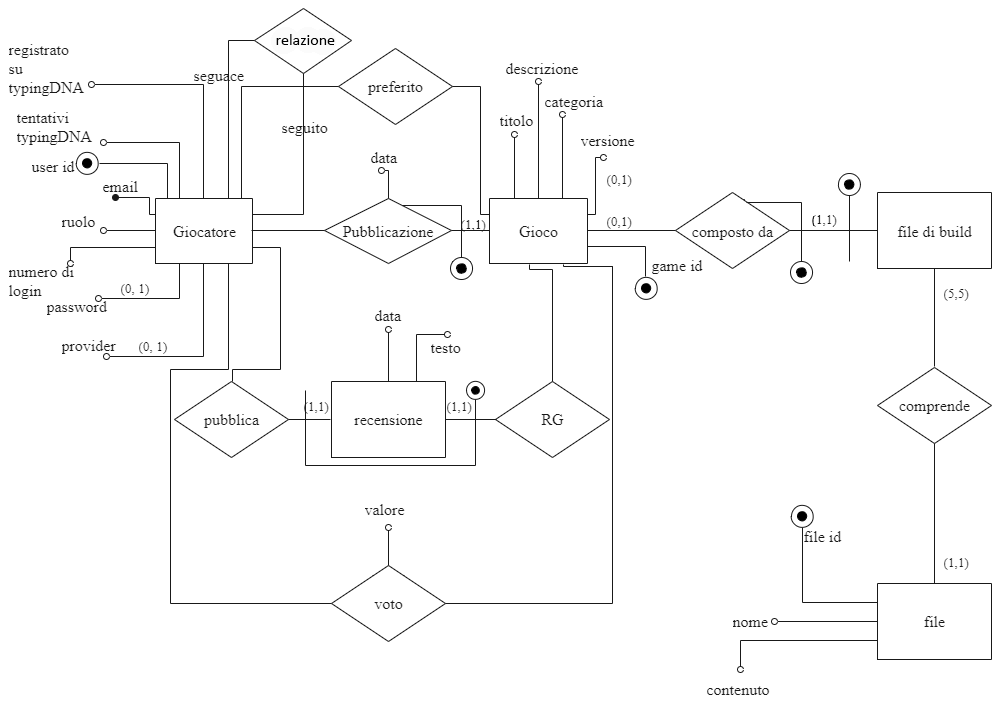
\includegraphics[angle=-90, width=\textwidth]{schemaER_ristrutturato}
    \caption{Schema ER ristrutturato}
\end{figure}

\begin{figure}[hbt!]
    \centering
    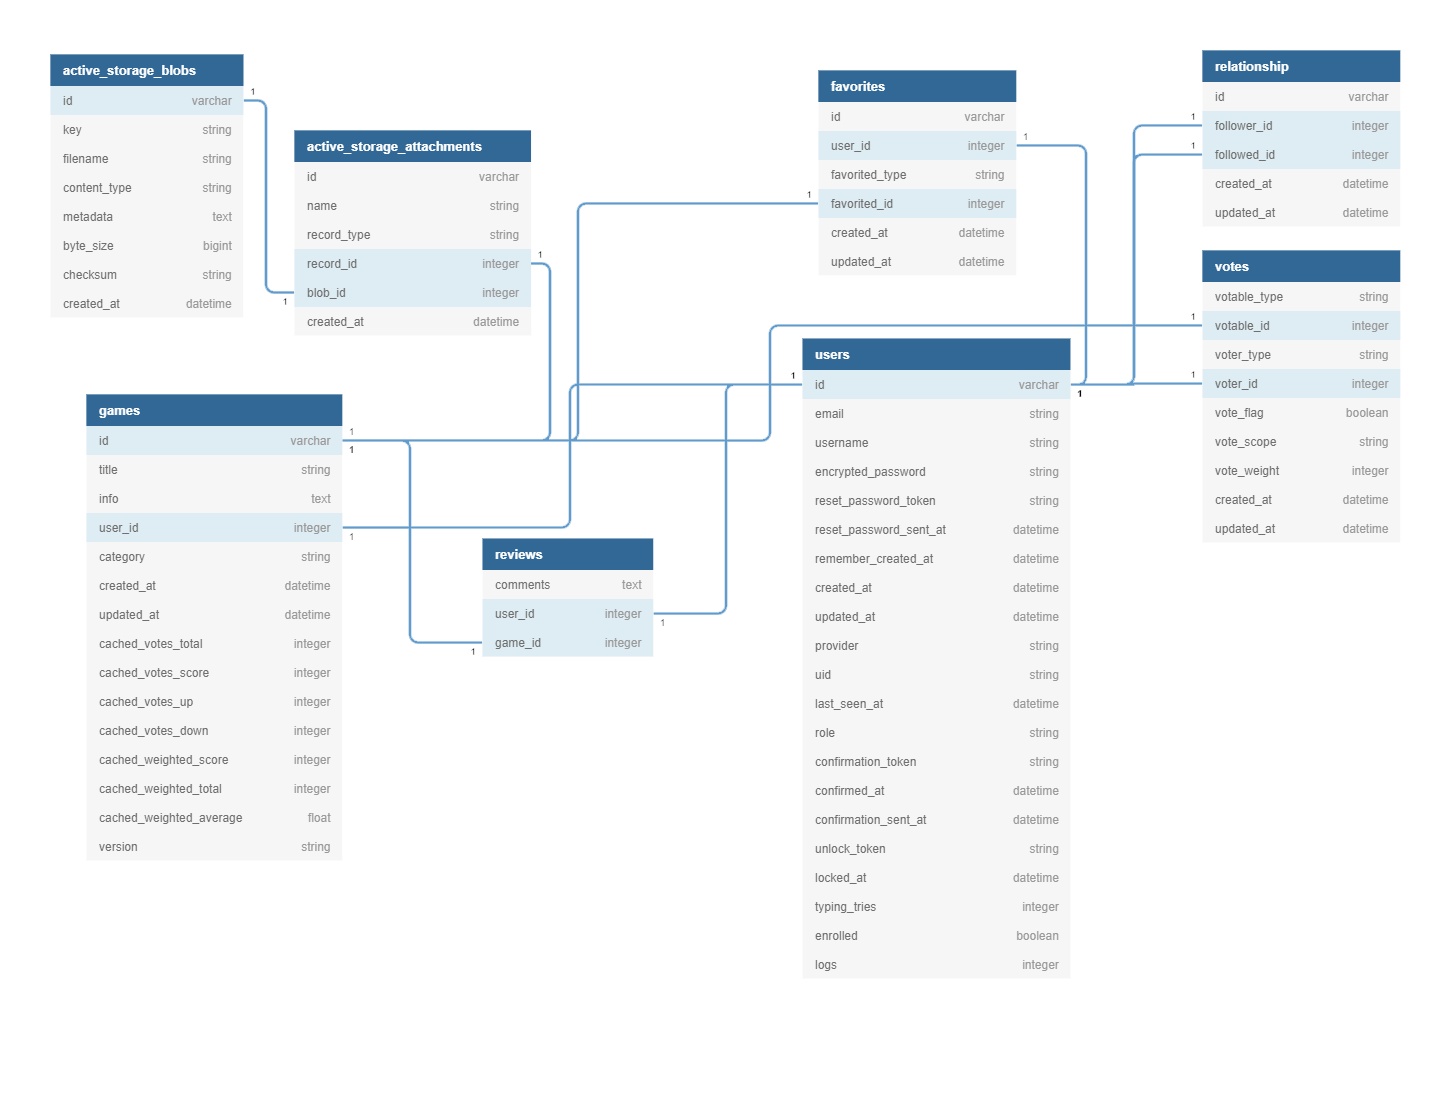
\includegraphics[angle=-90, width=\textwidth]{schema_relazionale}
    \caption{Schema relazionale}
\end{figure}

\FloatBarrier
\section{Architettura dell'applicativo software}
L'approccio \emph{Model-View-Controller} si presta alla realizzazione di applicativi web.\cite{ProgSoft} L'applicazione viene divisa in tre parti: modelli (che si occupano di memorizzare e stabilire le regole sui dati), viste (che presentano i dati e le operazioni disponibili agli utenti) e controllori (che fa da intermediario tra modelli, viste e utente finale), permettendo così di isolare il codice che gestisce i dati da quello che li presenta agli utenti.\\

\subsection{Gestione dei dati}
Per poter memorizzare i dati in un database SQL e contemporaneamente usare l'architettura MVC è necessario collegare le due realtà attraverso librerie di tipo \emph{Object-Relational Mapping} (ORM).\\

Grazie a queste librerie è possibile assegnare ad ogni tabella una classe, ad ogni riga un oggetto della classe, ai valori delle colonne gli attributi degli oggetti. Le query da effettuare sul DB vengono invocate attraverso metodi forniti dalle classi.\\

La seguente immagine mostra il diagramma delle classi per l'applicazione. Ad ogni classe corrisponde un modello.\\

\begin{figure}[hbt!]
    \centering
    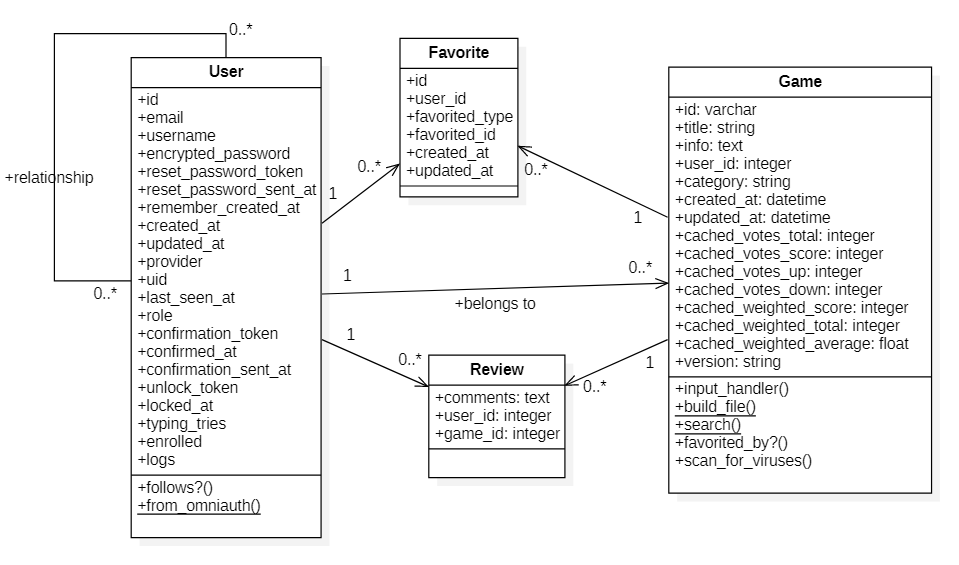
\includegraphics[width=\textwidth]{UML.png}
    \caption{Diagramma UML}
\end{figure}

\FloatBarrier
\subsection{Logica dell'applicazione e presentazione}
Come accennato in precedenza, la logica dell'applicazione viene gestita dai controllori. I controllori recuperano i dati dai modelli e li forniscono alle viste per accessi in lettura, viceversa per modifiche ai dati\footnote{Occorre tenere presente che la vera e propria modifica ai dati viene effettuata dai modelli. I controllori comunicano solo cosa fare.}.\\

Di seguito sono riportati i vari schemi che mostrano come i vari controllori comunicano alle viste i dati da presentare prendendoli dai modelli\footnote{Questi schemi, anche se hanno a che fare con l'architettura vera e propria, intendono essere molto astratti, per rendere la loro lettura il più semplice possibile. La comunicazione, infatti, tra modelli, controllori e viste è più complessa e sotto certi aspetti la lettura diretta del codice renderebbe meglio l'idea.}. Le frecce continue rappresentano la provenienza dei dati dai modelli alle viste attraverso i controllori. Le frecce tratteggiate servono ad indicare una derivazione di un controllore rispetto ad un altro. Dato che tutti i controllori estendono l'\emph{application controller} le frecce tratteggiate corrispondenti sono sottintese. Per semplicità non sono stati inseriti negli schemi i controllori intermediari relativi alla gemma \emph{devise}.

\begin{figure}[hbt!]
    \centering
    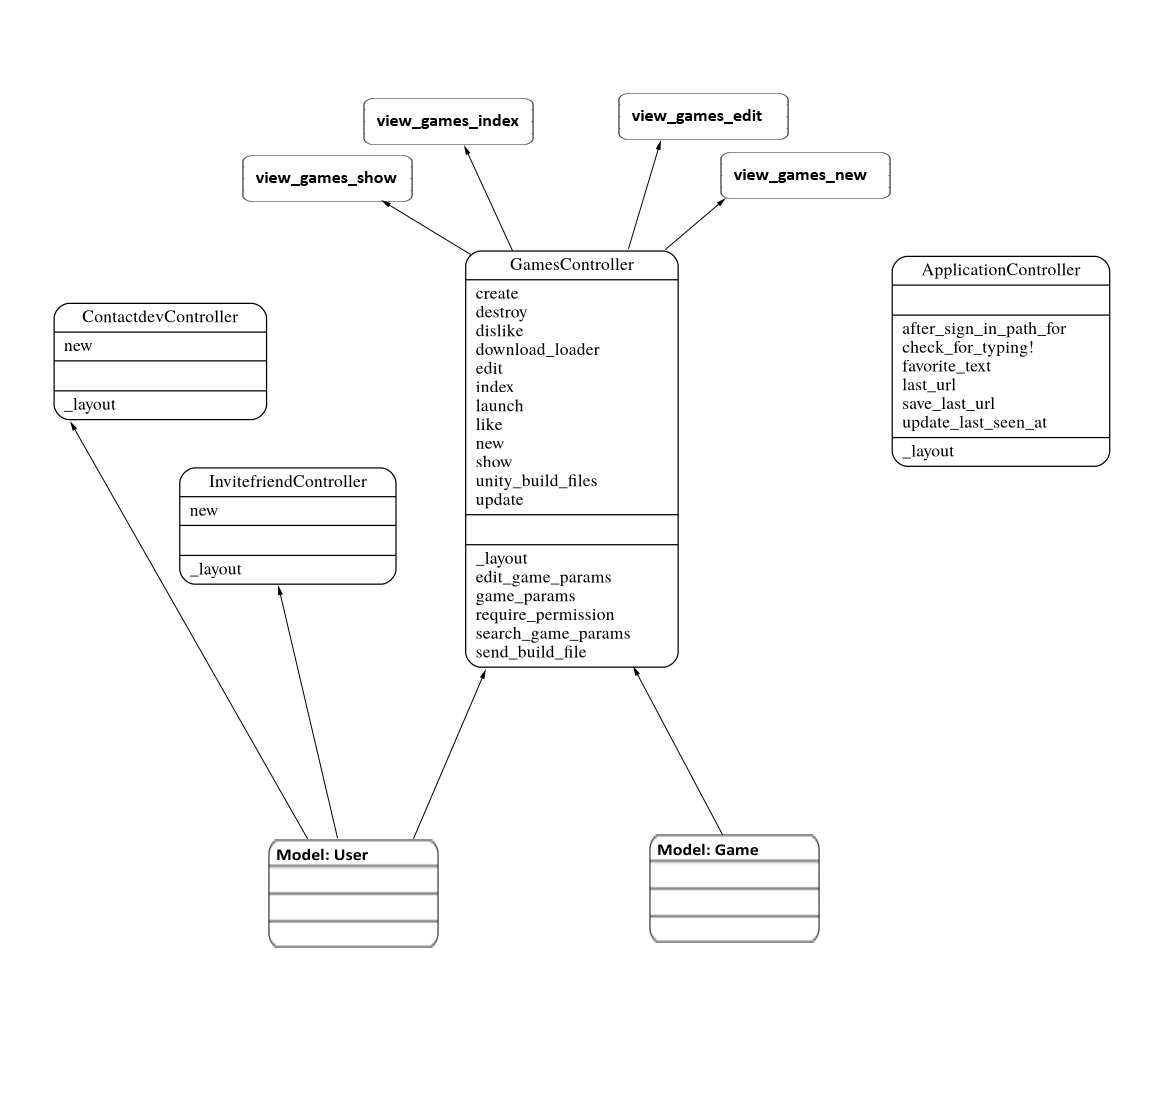
\includegraphics[width=\textwidth]{games_controller.png}
    \caption{GamesController}
\end{figure}

\begin{figure}[hbt!]
    \centering
    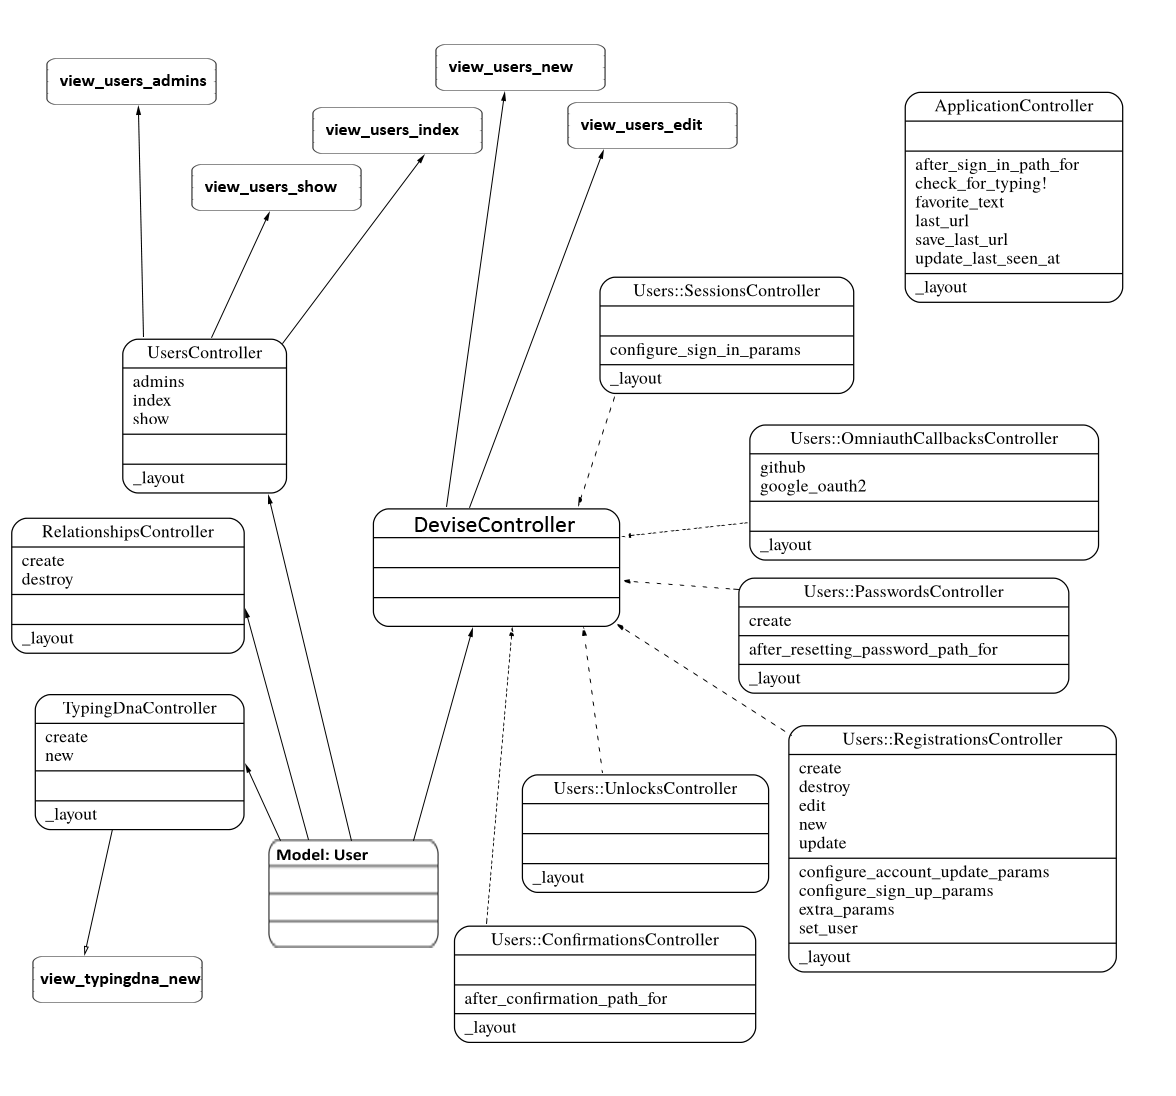
\includegraphics[width=\textwidth]{users_controller.png}
    \caption{UsersController}
\end{figure}
\FloatBarrier
\footnote{\emph{view\_users\_edit} è da intendersi come comprensiva di tutte le viste che presentano campi per modificare gli utenti.}

\begin{figure}[hbt!]
    \centering
    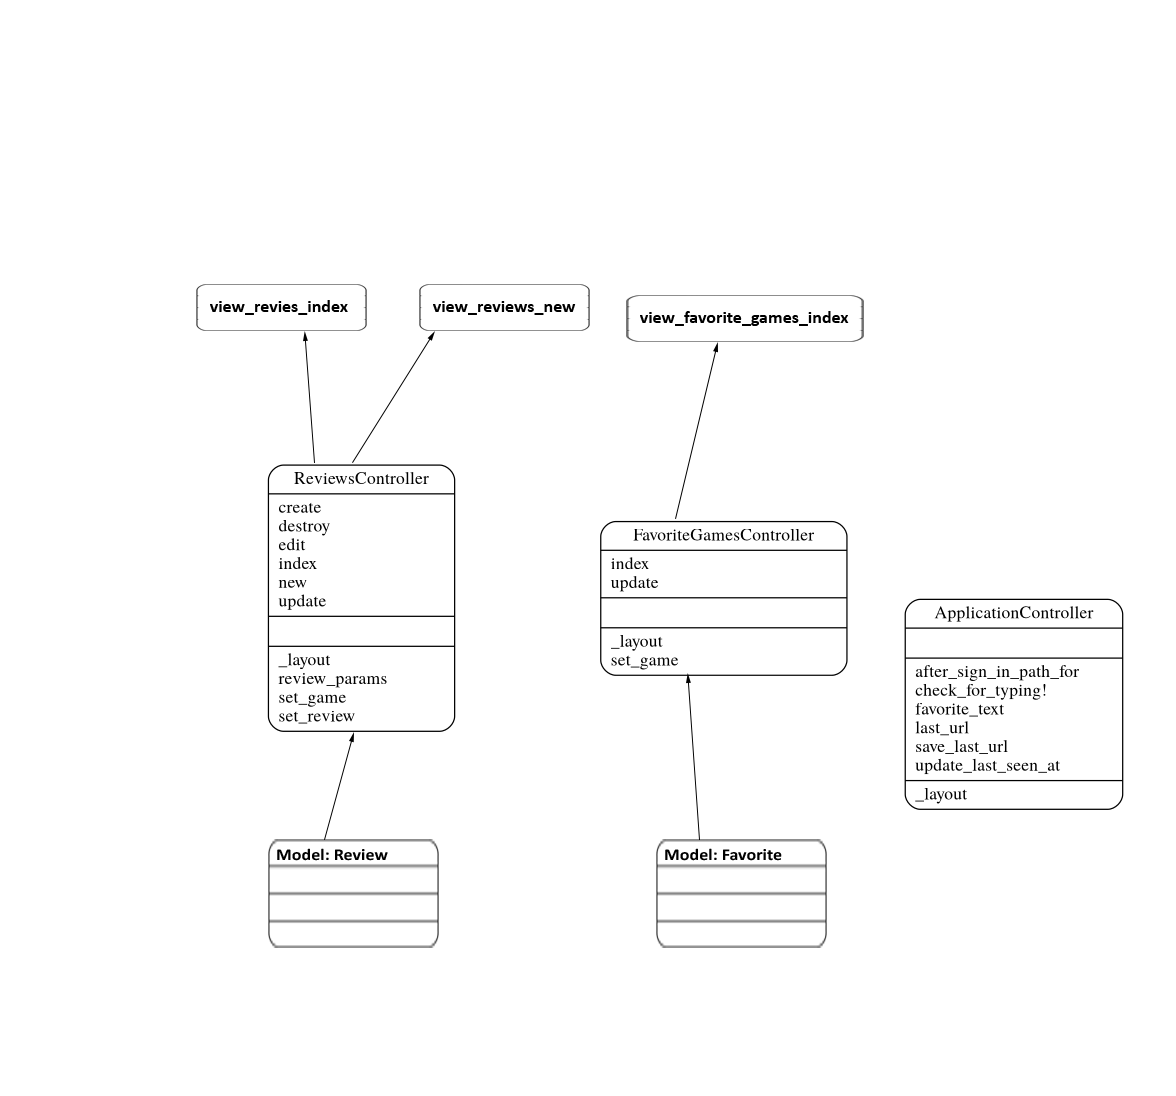
\includegraphics[width=\textwidth]{reviews_favorites_controller.png}
    \caption{ReviewsController e FavoriteGamesController}
\end{figure}

\chapter{Studio di un caso d'uso}
In questo capitolo sarà analizzato un caso di utilizzo dell'applicazione. Per farlo saranno utilizzati i \emph{diagrammi delle attività} e i \emph{diagrammi di sequenza}. Il caso d'uso di interesse è quello della pubblicazione di un gioco, partendo dalla fase di autenticazione\footnote{In ogni caso è possibile eseguire il codice scaricandolo da \url{https://github.com/davidebazzana/game\_on} al branch giacomo}.\\

\section{Accesso al sistema}
Quando un utente intende pubblicare un nuovo gioco, nel caso non sia autenticato, l'applicazione lo reindirizza alla pagina di login. Effettuato il login correttamente l'utente potrà pubblicare il gioco compilando l'apposito form.\\
Il seguente diagramma delle attività descrive la fase di login.
\begin{figure}[H]
    \centering
    \includegraphics[width=0.8\textwidth]{diagramma_attività_autenticazione}
    \caption{Diagramma attività: autenticazione utente}
\end{figure}

\FloatBarrier
Quest'altro diagramma mostra la pubblicazione vera e propria del gioco.\\
\begin{figure}[hbt!]
    \centering
    \includegraphics[width=\textwidth]{diagramma_attività_nuovo_gioco}
    \caption{Diagramma attività: pubblicazione nuovo gioco}
\end{figure}
\FloatBarrier
A livello informatico vero e proprio la sequenza di eventi relativa all'autenticazione di un utente e alla successiva pubblicazione di un gioco può essere rappresentata dal seguente diagramma di sequenza. Nel caso considerato si ipotizza che l'utente riesca ad autenticarsi al primo tentativo, che però debba verificare la sua identità attraverso typingDNA e che nella creazione del gioco non abbia compiuto alcun errore né abbia tentato di caricare un virus.\\
\begin{figure}
    \centering
    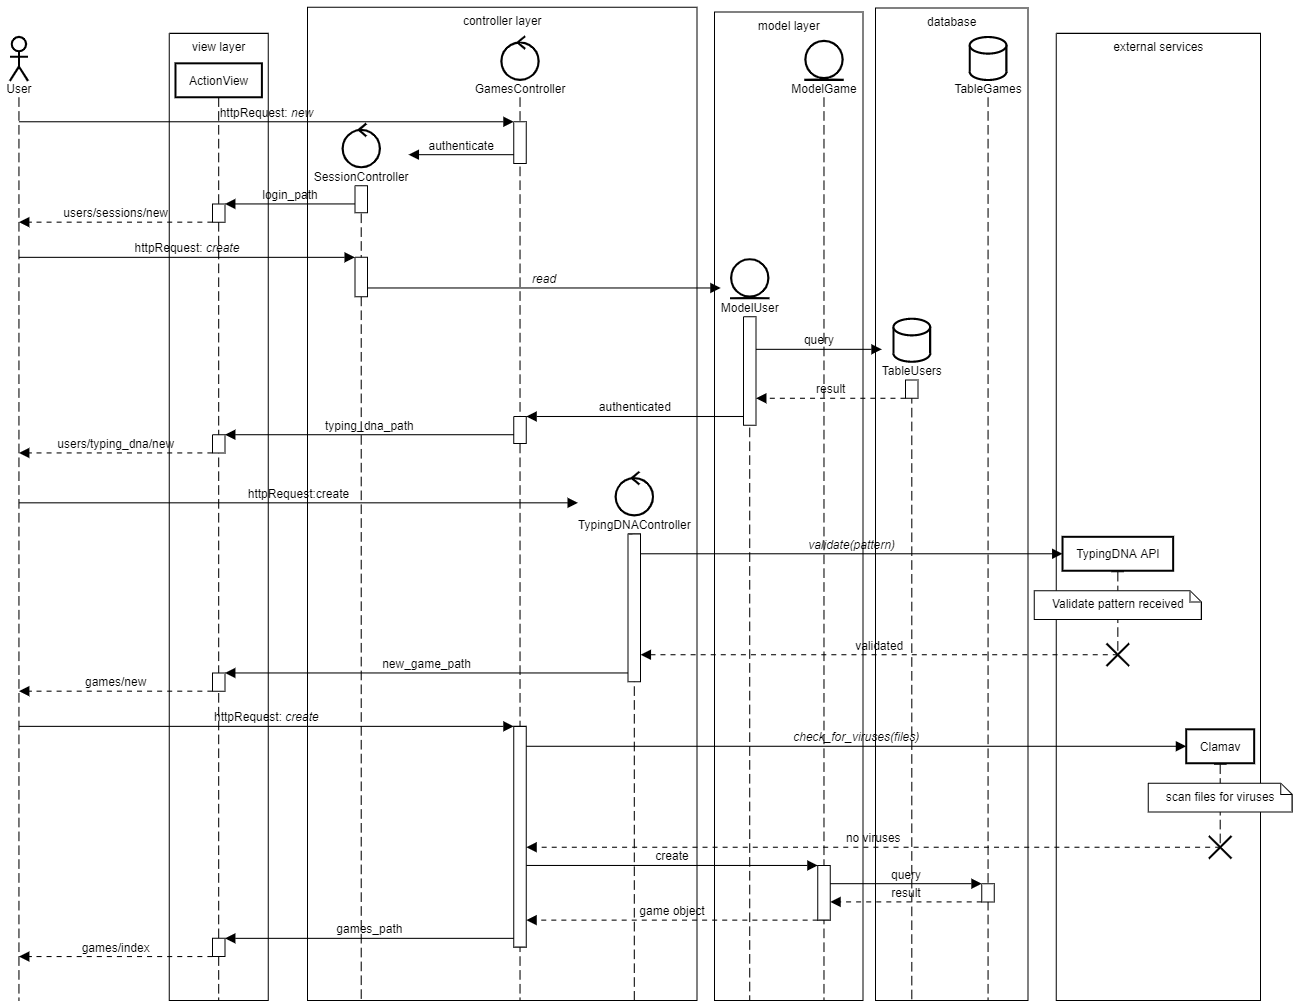
\includegraphics[width=1.2\textwidth]{new_game_sequence_diagram}
    \caption{Diagramma di sequenza: autenticazione e pubblicazione gioco}
\end{figure}

\chapter{Test e validazione del software}
Il \emph{testing} del software è un procedimento utilizzato per individuare errori e potenziali migliorie nel software in corso di sviluppo. La ricerca di questi aspetti contribuisce alla buona qualità del prodotto.\cite{test}\\

La fase di validazione invece, serve ad assicurarsi che il software rispecchi i requisiti richiesti in partenza. Può essere fatta staticamente, analizzando il codice, o dinamicamente, collaudandolo con dati di test.\\

Adesso sarà mostrato l'approccio BDD\footnote{BDD consiste in una serie di passaggi da seguire ciclicamente: \begin{itemize}
    \item Identificare le funzionalità del software.
    \item Identificare gli scenari sotto la funzionalità selezionata.
    \item Definire i passaggi per ogni scenario.
    \item Eseguire la funzionalità e fallire.
    \item Scrivere il codice per superare i test.
    \item Eeseguire la funzionalità e passare i test.
    \item Generare i resoconti dei test
\end{itemize}} (Behavior Driven Development) ad una user story presentata nel capitolo 2.\\

\emph{Come giocatore proprietario di un gioco, voglio modificare il gioco, così che lo possa mantenere aggiornato.}\\

Il codice seguente mostra il file ChangeGame.feature. La prima riga definisce la funzionalità testata. Gli step definiti (identificati da \emph{Given, When, Then}), permettono che gli scenari corrispondenti possano essere eseguiti e sono scritti in modo da rispecchiare il più possibile la definizione della user story corrispondente.\\

\newpage
\begin{lstlisting}[language=Gherkin]
Feature: The owner of a game can change a game

Background:
        Given I am a registered user

Scenario: Change the title of a game
    Given I am the owner of the game "old_title"
        When I follow "More about old_title"
    And I follow "Edit game"
    And I fill in "Title" with "new_title"
    And I click on "Commit updates"
    Then I should be on the Game-on home page
    And I should see "new_title", not "old_title" anymore

Scenario: Change the description of a game
    Given I am the owner of the game 
        "game_title" with info "old_info"
    When I follow "More about game_title"
    And I follow "Edit game"
    And I fill in "Info" with "new_info"
    And I click on "Commit updates"
    And I follow "More about game_title"
    Then I should see "new_info", not "old_info" anymore


Scenario: Change the title and the description of a game
        Given I am the owner of the game 
            "old_title" with info "old_info"
    When I follow "More about old_title"
    And I follow "Edit game"
    And I fill in "Title" with "new_title"
    And I fill in "Info" with "new_info"	  
    And I click on "Commit updates" 
    And I follow "More about new_title"
    Then I should see "new_title", not "old_title" anymore
    And I should see "new_info", not "old_info" anymore
\end{lstlisting}

Lo strumento utilizzato per analizzare il codice appena visto si chiama \emph{Cucumber}. In pratica per ogni step verrà cercata una definizione in Rby corrispondente tra i file all'interno della cartella predefinita "step\_definitions". Ecco la definizione degli step sopra riportati.\\

\begin{lstlisting}[language=Ruby]
Given("I am a registered user") do
  visit "http://www.example.com/signup"
  fill_in "Email", :with => "test_user@example.com"
  fill_in "Username", :with => "test_user"
  fill_in "Password", :with => "password_001"
  fill_in "Password confirmation", :with => "password_001"
  click_button("Sign up")
  open_email("test_user@example.com")
  visit_in_email("Confirm my account", 
    "test_user@example.com")

  @test_user_email = "test_user@example.com"
end

Given("I am the owner of the game {string}") do |game_title|
  create(:game, title: game_title, 
  user_id: User.find_by_email(@test_user_email)[:id])
end

When("I follow {string}") do |link|
  visit current_url
  click_link(link)
end

When("I fill in {string} with {string}") do |field, content|
  fill_in field, :with => content

  @test_user_email = content if field.eql?("Email")
end

When("I click on {string}") do |button|
  click_button(button)
end

Then("I should be on the Game-on home page") do
  expect(current_url).to eq("http://www.example.com/games")
end

Then("I should see {string}, 
    not {string} anymore") do |new_value, old_value|
  expect(page).to have_content(new_value)
  expect(page).to have_no_content(old_value)
end

Given("I am the owner of the game {string} 
    with info {string}") do |game_title, info|
  create(:game, title: game_title, 
    user_id: User.find_by_email(@test_user_email)[:id], info: info)
end
\end{lstlisting}

Per quanto riguarda i test si usa l'approccio TDD (Test-driven Development), che permette di creare un framework di base per l'esecuzione del codice che verrà scritto successivamente. In pratica i test vengono prima del codice vero e proprio. Per implementare tutto ciò si usa \emph{RSpec}, che permette di scrivere tesi in Ruby.\\

L'esempio seguente mostra il codice di test per la funzionalità di ricerca tra i giochi:

\begin{lstlisting}[language=Ruby]
require 'spec_helper'

RSpec.describe "Games", type: :request do
    games = [{:title => "Pet em all", :category => "Other"},
            {:title => "Cats island", :category => "Other"},
            {:title => "Dogcatcher simulator", 
                :category => "Other"},
            {:title => "Sleeping cat", 
                :category => "Other"},
            {:title => "Cat race", :category => "Racing"},
            {:title => "Purring cat", 
                :category => "Casual"},
            {:title => "Mreow", :category => "Casual"}]

    all_games = Array.new()
    cats_games = Array.new()
    casual_games = Array.new()
    casual_cats_games = Array.new()
    
    FactoryBot.create(:user, :username => "Thelonious", 
        :email => "thelonious@email.com")
    games.each do |game|
    new_game = FactoryBot.create(:game, :title => game[:title], 
        :category => game[:category])
    all_games.append(new_game)
    if(game[:title].downcase().include?("cat"))
        cats_games.append(new_game)
    end
    if(game[:category].include?("Casual"))
        casual_games.append(new_game)
    end      
    if(game[:title].downcase().include?("cat") && 
        game[:category].include?("Casual"))
        casual_cats_games.append(new_game)
    end
    end

    describe "Search by name" do
    it "Search for all the games with 'cat' in their name" do
        allow(Game).to 
            receive(:search).and_return(cats_games)
        get '/games', :params => {:game => {:title => "cat", 
            :category => "Any", :sort_criterion => "Any"}}
        expect(response).to be_successful
        expect(response).to have_http_status(:success)
        cats_games.each do |game|
        expect(response.body).to include(game[:title])
        end
    end
    end

    describe "Search by category" do
    it "Search for all the games with category 'Casual'" do
        allow(Game).to 
            receive(:search).and_return(casual_games)
        get '/games', :params => {:game => {:title => "", 
            :category => "Casual", :sort_criterion => "Any"}}
        expect(response).to be_successful
        expect(response).to have_http_status(:success)
        casual_games.each do |game|
        expect(response.body).to include(game[:title])
        end
    end
    end

    describe "Search by name and category" do
    it "Search for all the games" do
        allow(Game).to 
            receive(:search).and_return(all_games)
        get '/games', :params => {:game => {:title => "", 
            :category => "Any", :sort_criterion => "Any"}}
        expect(response).to be_successful
        expect(response).to have_http_status(:success)
        all_games.each do |game|
        expect(response.body).to include(game[:title])
        end
    end
    
    it "Search for all the games with 'cat' in their name 
        and with category 'Casual'" do
        allow(Game).to 
            receive(:search).and_return(casual_cats_games)
        get '/games', :params => {:game => {:title => "cat", 
            :category => "Casual", :sort_criterion => "Any"}}
        expect(response).to be_successful
        expect(response).to have_http_status(:success)
        casual_cats_games.each do |game|
        expect(response.body).to include(game[:title])
        end
    end
    end
end    
\end{lstlisting}



\chapter{Le \emph{behavioral biometrics} come futuro dell'autenticazione}
Nel corso della tesi è stato fatto riferimento più volte a typingDNA e alle behavioral biometrics. Ma cosa sono esattamente? Quali sono le applicazioni e le potenzialità in termini di sicurezza informatica? Questo capitolo si occuperà di rispondere a queste domande.\\

\section{Cosa si intende con behavioral biometrics}
Le behavioral biometrics, in italiano parametri biometrici comportamentali, sono dati relativi all'uso che ogni persona fa dei suoi dispositivi, concentrandosi più su \emph{come} vengono svolte determinate azioni, che su \emph{quali} esse siano.\\
Per esempio, quasi ogni possessore di un dispositivo elettronico ha accesso ad un qualche servizio di posta elettronica e probabilmente controllerà ogni giorno le nuove email ricevute e a vote ne scriverà di sue. Ma è molto probabile che non tutti gli utenti di tale servizio aprano le email con la stessa velocità, scorrano con la rondella del mouse o col dito allo stesso modo, abbiano la stessa rapidità e accuratezza nel digitare sulla tastiera.\\
Con l'utilizzo sempre maggiore del \emph{machine learning} e dell'intelligenza artificiale è possibile immagazzinare ed elaborare le informazioni elencate sopra (e molte altre) per costruire un profilo univoco della persona che utilizza tali servizi.\\
I classici metodi per tenere in sicurezza i propri account sono ormai decadenti. Le password molto raramente vengono scelte con criteri di sicurezza elevati e comunque molti utenti decidono di salvarle all'interno del browser o attraverso un servizio di memorizzazione password. Accedendo al servizio principale sarebbe quindi possibile accedere a tutte le password dell'utente con conseguenze evidentemente gravi.\\
L'autenticazione a due fattori, che viene sempre più utilizzata, fornisce un alto livello di sicurezza, ma comunque richiede dei passaggi attivi da parte dell'utente, per essere applicata e non sarebbe pratico richiederla per ogni accesso ad un servizio.\\
Anche i parametri biometrici veri e propri (scansione dell'impronta digitale, del volto, dell'iride) sono metodi di autenticazione sicurissimi, ma richiedono componenti hardware specifiche e non sono utilizzabili in ogni situazione con comodità.\\
Se, invece, i dispositivi fossero in grado di riconoscere il proprio possessore confrontando il suo comportamento attuale con quello avuto in passato (o ancora meglio, riconoscere un tentativo di utilizzo da parte di un individuo esterno), allora potrebbe essere sempre possibile verificare l'identità dell'utente senza che lui debba compiere alcun gesto se non quelli che aveva già previsto di dover compiere. Questo sistema permetterebbe ai dispositivi e ai servizi di essere molto più \emph{user friendly}.\\
C'è da dire che costruire un profilo comportamentale per ogni individuo può spaventare molte persone, ma è opportuno tener presente che attualmente già vengono registrate molte informazioni personali su di noi. I movimenti tracciati via GPS, i passi che effettuiamo ogni giorno e potenzialmente anche il nostro modo di camminare, i battiti cardiaci e tanto altro. Sicuramente però utilizzare i dati personali comportamentali nei modi suddetti può contribuire alla sicurezza di questi stessi dati!


\section{Il servizio TypingDNA}
All'interno di \emph{Game on} ho deciso di utilizzare il servizio TypingDNA\cite{tdna} perché fornisce una dimostrazione molto semplice, ma efficace, delle potenzialità nell'utilizzo delle behavioral biometrics.\\
Con TypingDNA è possibile riconoscere un utente attraverso il suo modo di digitare su una tastiera (sia su desktop che su smartphone).\\
Il suo utilizzo è molto semplice: 
\begin{itemize}
    \item Lato client viene registrato lo stile di digitazione dell'utente grazie alla libreria javascript \emph{typingdna.js}. I parametri vengono salvati sotto forma di \emph{pattern}.
    \item Lato server il pattern ottenuto viene preso e rilanciato attraverso una chiamata REST alla REST API sui server di TypingDNA.
    \item TypingDNA risponde con un json che comunicherà la validità o meno del pattern fornito
\end{itemize}
\begin{figure}[hbt!]
    \centering
    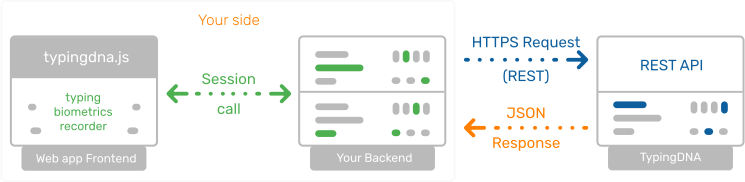
\includegraphics[width=\textwidth]{typingDNA_workflow}
    \caption{Workflow di TypingDNA}
\end{figure}
\FloatBarrier
Le API messe a disposizione permettono di verificare tre tipi di pattern: \emph{same text} autentica basandosi sulla digitazione dello stesso testo; \emph{any text} autentica basandosi sulla digitazione di testi sempre diversi; \emph{extended text} è una combinazione dei precedenti.
\subsection{Utilizzo di TypingDNA all'interno dell'applicazione}
All'interno di Game on sono stati implementati diversi controlli attraverso typingDNA: 
\begin{itemize}
    \item Un pattern \emph{same text} viene utilizzato con la mail dell'utente nei primi accessi al sito e successivamente ogni 10 login. L'utente ha 3 tentativi per entrare, dopo i quali l'account viene bloccato e una mail di recupero viene inviata all'utente.
    \item Un pattern \emph{any text} viene creato quando un utente scrive una recensione o la descrizione di un gioco e la lunghezza del testo è sufficientemente lunga. In caso di fallimento l'utente è sospetto e viene reindirizzato alla pagina di inserimento mail descritta sopra.
\end{itemize}

\backmatter
\cleardoublepage
\phantomsection
\addcontentsline{toc}{chapter}{\bibname}
\printbibliography
	
\end{document}
